% ============================================================
% Gemma 3 replication -- ADDITION TO main_final.tex, kept separate for review.
%
% Suggested placement:
%   * Section "Replication on Gemma 3 with pre-trained dictionaries" goes after
%     Section 3.4 ("Downstream re-reading does not explain the ceiling") and
%     before the Discussion, as Section 3.5.
%   * The appendix section goes after Appendix D.
%   * Figures: gemma3_4b_fig1_knockout_landscape, gemma3_4b_fig_decomposition,
%     gemma3_4b_fig6_budget_distribution, gemma3_4b_fig8a_ablation_vs_knockout,
%     gemma3_4b_fig8b_recovered_share, gemma3_4b_fig_single_layer, in
%     paper_figures/ (PNG + PDF).
%   * Bibliography entries to append to refs.bib are at the end of this file.
%   * Suggested one-sentence changes to the abstract and to the Limitations
%     paragraph are given as comments at the end.
%
% Every number below is read from committed artifacts of the vlm-flow-probe
% repo (output/experiments/gemma3_4b_*; see docs/gemma3_replication.md there
% for the run log and the decision record). n = 256 conditions all share the
% same first-256 validation questions in the same order (SHA-1 verified by
% the analysis), so paired statements hold as in the LLaVA runs.
% ============================================================

% ------------------------------------------------------------
% Self-compiling guard.  If this file is compiled on its own (Overleaf's
% "main document"), it loads a class and opens the document environment; if it
% is \input into main_final.tex, the class is already loaded and the whole
% block is skipped.  Keep it -- without it a solo compile produces no PDF
% ("the document environment contains no content").
% ------------------------------------------------------------
\expandafter\ifx\csname @classoptionslist\endcsname\relax
  \documentclass[11pt,a4paper]{article}
  \usepackage[T1]{fontenc}
  \usepackage{lmodern}
  \usepackage[margin=2.5cm]{geometry}
  \usepackage{amsmath,amssymb}
  \usepackage{graphicx}
  \usepackage{booktabs}
  \usepackage{multirow}
  \usepackage{array}
  \usepackage{hyperref}
  \usepackage{xcolor}
  \usepackage{microtype}
  \usepackage{parskip}
  \usepackage[round]{natbib}
  \graphicspath{{paper_figures/}{figures/}}
  \begin{document}
  \newcommand{\gemmastandalone}{}
\fi

\section{Replication on Gemma 3 with pre-trained dictionaries}
\label{sec:gemma}

The calibration above rests on three premises that the LLaVA setup satisfied
without being stated: the dictionary reconstructs the site it is applied to,
the features it selects act on the pathway the knockout severs, and the margin
is far from saturation so that its drop measures loss of the answer. We
re-ran the full design on a second model whose dictionaries we did not train,
Gemma~3 4B with Gemma~Scope~2's attention SAEs, and found all three premises
violated in ways that the design detects but cannot repair. We report it as a
boundary-conditions result: what the calibration requires, and what its numbers
look like when the requirements fail.

\paragraph{Setup.} Gemma~3 4B (instruction-tuned) \citep{gemma3}: a SigLIP
encoder pooled to 256 image tokens, and a 34-layer decoder
($d_{\text{model}} = 2560$; eight heads of width 256) in which every sixth
layer (5, 11, 17, 23, 29) attends globally and the rest attend within a
1{,}024-token window --- wider than the 286-token CLEVR-Lite prompt, so every
layer sees the whole sequence. Dictionaries are Gemma~Scope~2's
\citep{gemmascope2} JumpReLU \citep{rajamanoharan2024jumprelu} attention SAEs,
one per layer, 16{,}384 features ($8\times$ the site) at the densest released
sparsity (nominal $L_0$ 60--120). They read the input of the attention output
projection $W_O$, the concatenated head outputs (2048-wide), one linear map
before the site the LLaVA dictionaries read; ablation there writes
$W_O\hat{x}$ into the residual stream in place of $W_O x$. Everything else is
held fixed: CLEVR-Lite, the same validation split and 256-question evaluation
set, the margin, gradient$\times$activation selection with $k=200$ per layer,
activation-matched controls, and the condition matrix. Four conventions had to
be set for the new model and are recorded in Appendix~\ref{app:gemma}: the
model answers with a capital letter (\texttt{Blue}) and scores the lowercase
string sixteen nats lower, so options are capitalised before scoring; the
language-model head is evaluated in float32 because bfloat16 quantises a
30-nat logit to steps of 0.125--0.25; question positions are every text
position after the image block, which is also what the LLaVA runs used in
effect (their question-token match never hit, so the fallback span applied;
recorded in the repository's adapter tests); and the feature scores are computed with the
dictionary's error term added back \citep{marks2024sparsefeaturecircuits}, so
the pass they are taken on is the unmodified model's.

\paragraph{The dictionaries do not fit the site.} Gemma~Scope~2 is trained on
text. On this task's question-position activations (203{,}245 rows from the
validation split) its attention dictionaries explain 67--95\% of the variance
(median 79\%; Table~\ref{tab:gemma-sae}), against 99.85--99.98\% for the
LLaVA dictionaries trained on the task, and 46--86\% of their features never
fire. \texttt{replace}-mode ablation, which substitutes the reconstruction for
the activation, is therefore unusable: with \emph{nothing} ablated it moves
the margin by $+1.56$ over layers 11--17 and by $-1.58$ over layers 16--17
(Appendix~\ref{app:gemma}), the size of a single-layer feature effect and of
either sign. All Gemma ablations below run in delta mode --- the activation
minus the selected features' decoded contribution --- for which the
zero-feature pass-through is exactly zero. This is the first place the design
diverges: the LLaVA study chose \texttt{replace} mode precisely so that a null
intervention would expose reconstruction error, and here the exposure is fatal
to that mode.

\paragraph{The landscape.} Figure~\ref{fig:gemma-landscape} gives the knockout
sweep over all 34 layers (Image$\rightarrow$Question on the 7{,}790
validation questions; the unmodified model answers every one of them
correctly, against 7{,}084 for LLaVA, so no filtering applies).
Transfer concentrates in a band, layers 11--17, with the global-attention
layer 17 far ahead (margin drop 5.58), then layer 0
(2.72), 12 (2.49), 11 (2.09), 15 and 14; an
isolated late site at layer 26 (1.60); and, unlike LLaVA,
\emph{inhibitory} layers in the majority --- blocking image attention raises
the margin at 17 of the 34 layers, substantially (by 0.4 or more) at 9, 16,
18, 21--25, 27, 32 and 33, and by 1.67 at layer 33. Image$\rightarrow$Last is near zero
everywhere except layer 26. The analysis span was fixed from the sweep before
any ablation ran, by the rule used for LLaVA: the contiguous band holding the
strongest sites other than layer 0, inhibitory members retained. That band is
seven layers here, 11--17, so the equal-budget point of the
spread-against-concentrated contrast is $40 \times 7 = 280$ features and
$k = 280$ was added to the concentrated curve.

\begin{figure}[t]
  \centering
  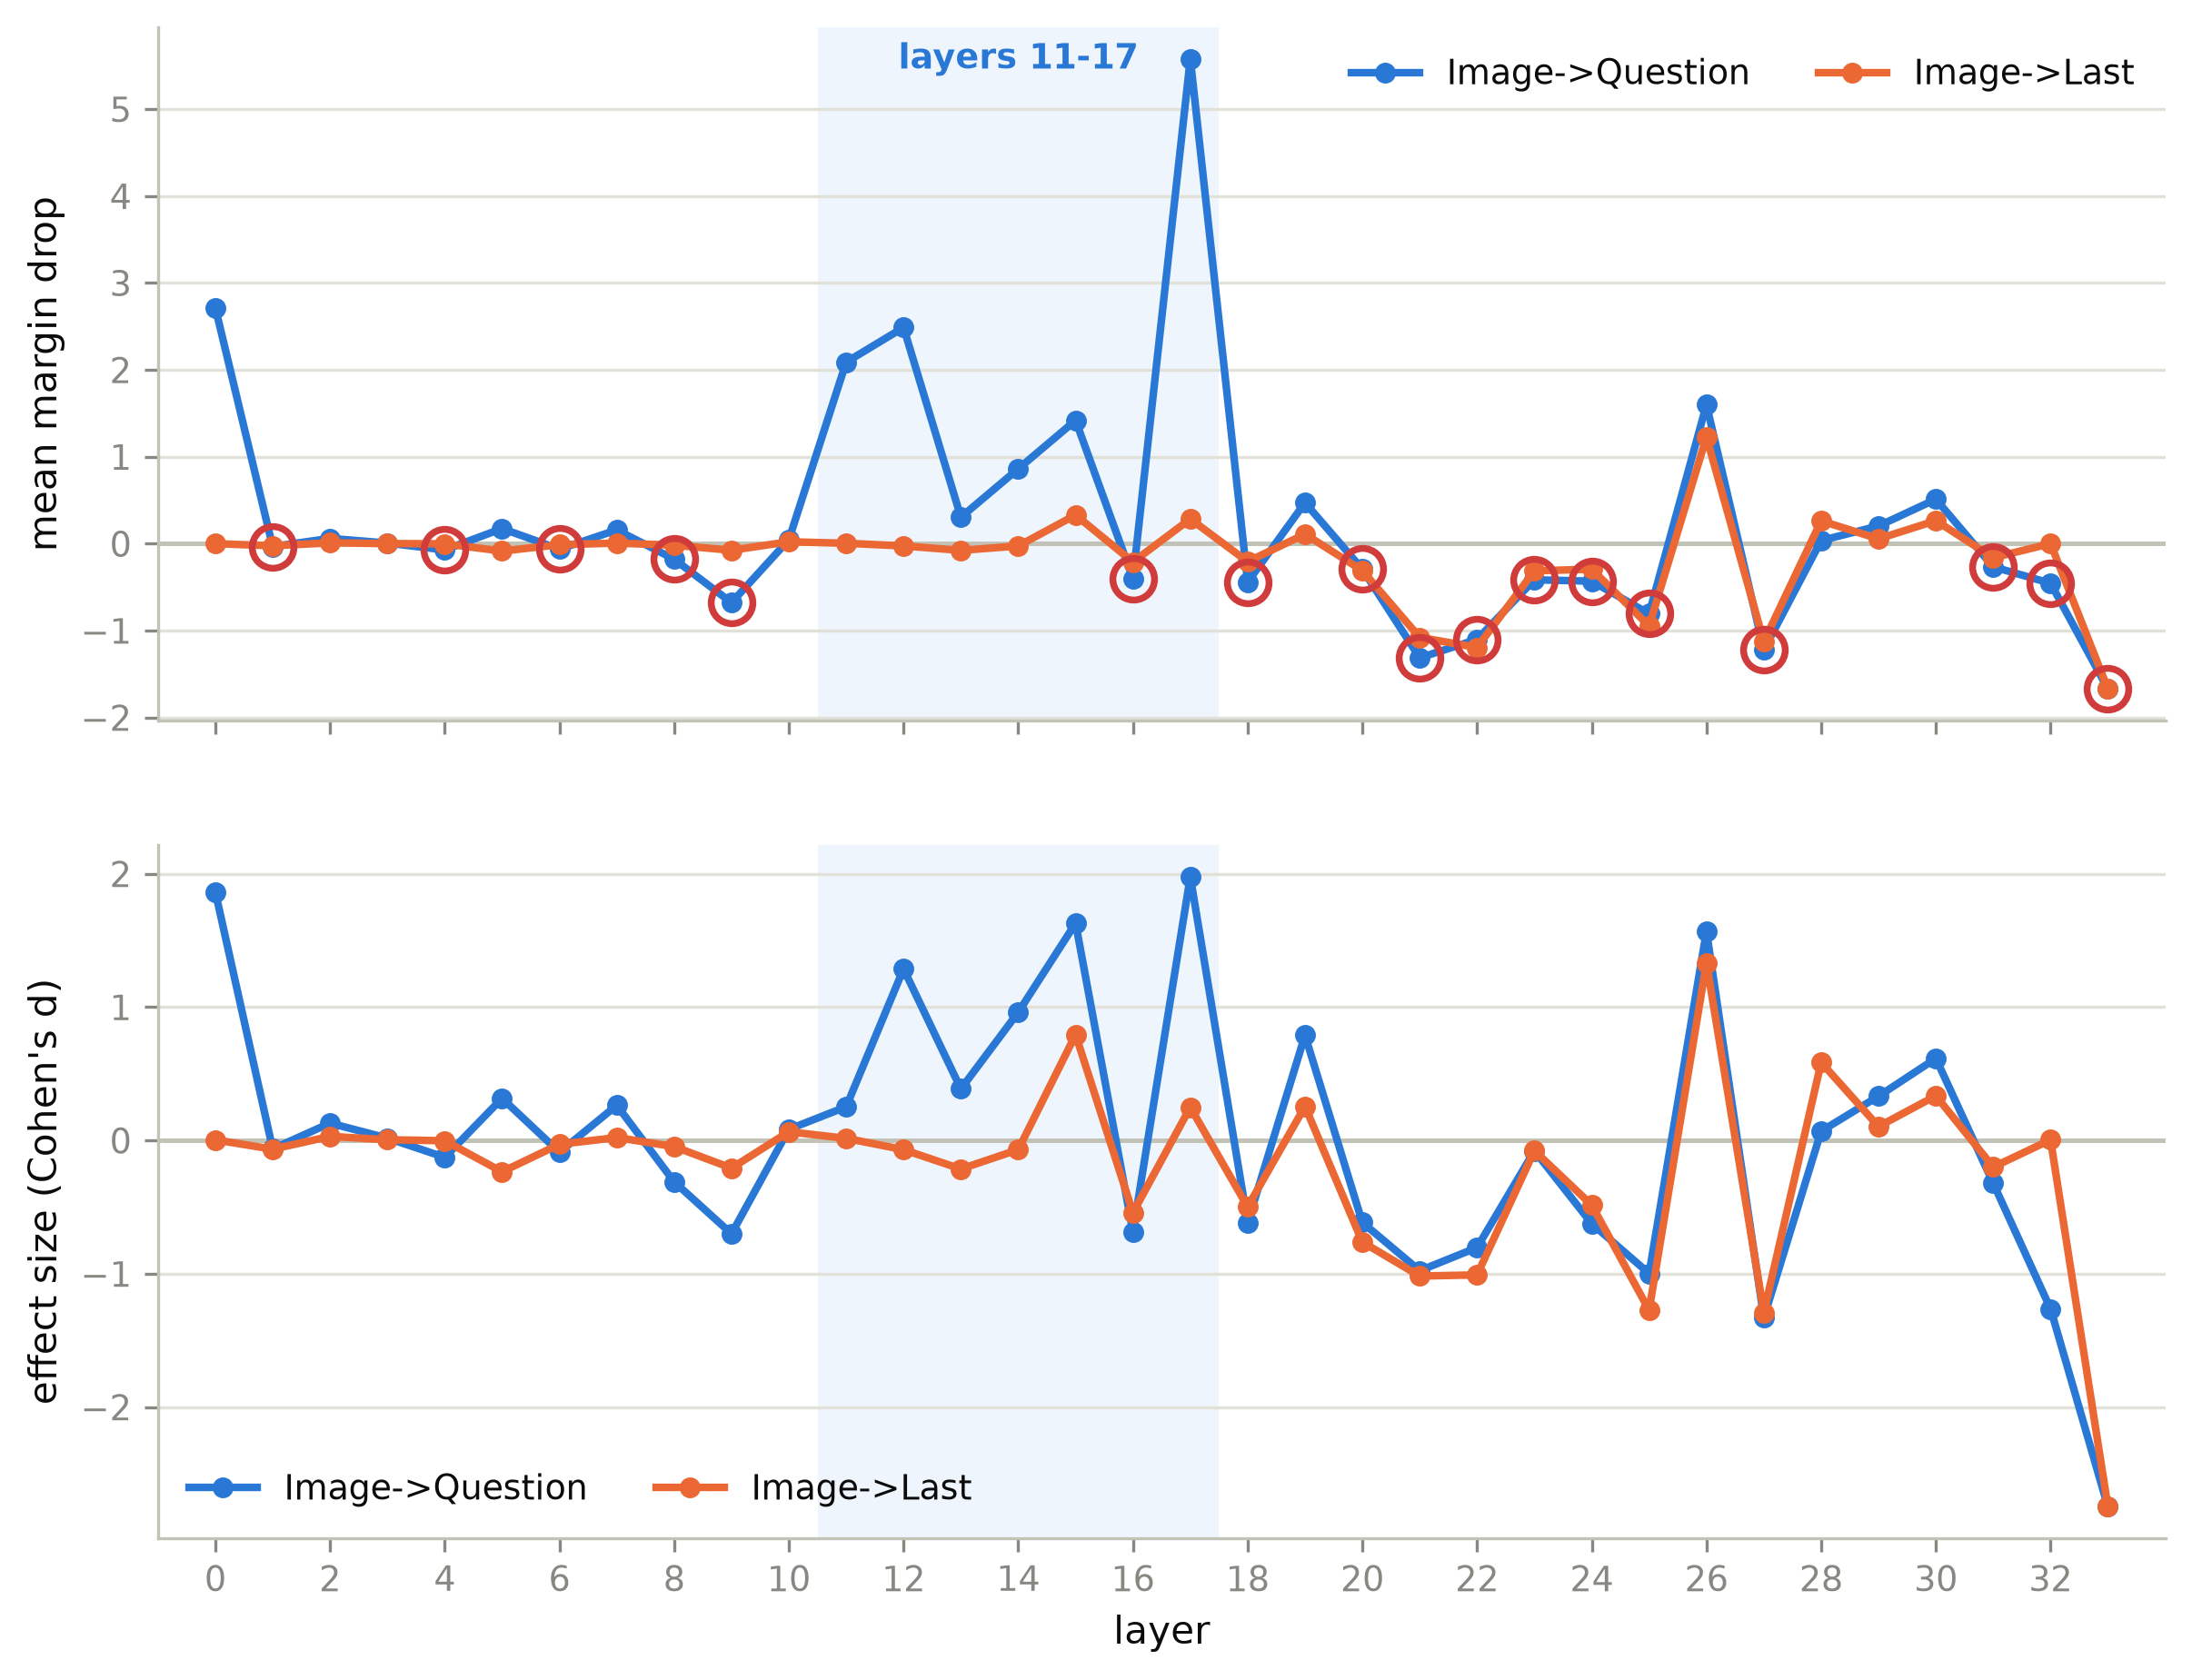
\includegraphics[width=\textwidth]{gemma3_4b_fig1_knockout_landscape}
  \caption{\textbf{Gemma~3 knockout landscape.} Mean margin drop (top) and
  Cohen's $d$ (bottom) from blocking Image$\rightarrow$Question (blue) and
  Image$\rightarrow$Last (orange) attention at each of the 34 decoder layers,
  $n = 7{,}790$. Ringed points are inhibitory. The shaded band marks
  layers 11--17, fixed as the analysis span from this sweep before any
  ablation was run.}
  \label{fig:gemma-landscape}
\end{figure}

\paragraph{Ablation and knockout do not track each other.} On LLaVA, single-layer
ablation fell below the knockout at every layer and the two ranked the layers
in the same order. On Gemma they are unrelated. Over all 34 layers, the top-200
ablation drop and the knockout drop rank-correlate at $\rho = 0.03$, and the
ablation exceeds the knockout at 23 of them. Within the span
(Table~\ref{tab:gemma-spans}), layer 12 has the second-strongest knockout
(2.55) and an ablation of 0.04; layer 16 has an inhibitory knockout ($-0.40$)
and the largest ablation of any layer (9.45); layer 17, the strongest knockout
(5.43), yields the one single-layer ratio that resembles LLaVA's,
$R = 39.9\%$ (95\% CI $[34.3, 45.6]$). Every other single-layer $R$ is above
2.8 or undefined. The controls are not the explanation: matched random sets
give 0.34 or less at every span layer, and the ablations are significant at
$z$ of 22 to 224.

\paragraph{The margin is saturated, and the two interventions move different
parts of it.} The unmodified model puts the true option at $\log P = -0.05$
and the false one at $-32.7$, a margin of 32.6 against LLaVA's 2.7. A drop can
then come from the true option falling or from the false option rising out of
the tail, and Figure~\ref{fig:gemma-decomp} separates them. Every single-layer
ablation effect, at all 34 layers, is false-option rise: the true option moves
by at most 0.02 nats and generation accuracy is unchanged at 0.996 (0.984 at
one layer). The single-layer knockouts are the same, with one exception ---
layer 11, where the true option falls by 0.97 nats on the 256-question set.
Even blocking Image$\rightarrow$Question at all seven span layers costs the
true option only 0.95 nats and leaves generation accuracy at 0.77: the model
still reads the image elsewhere (layer 0 and layer 26 among others), and
removing the answer requires cutting the 21 layers downstream of layer 12
(true-option drop 5.9, accuracy 0.19). The margin, in other words, is
reporting how sharply the model rejects the distractor far more than whether
it knows the answer, and at single layers neither intervention touches the
latter.

\begin{figure}[t]
  \centering
  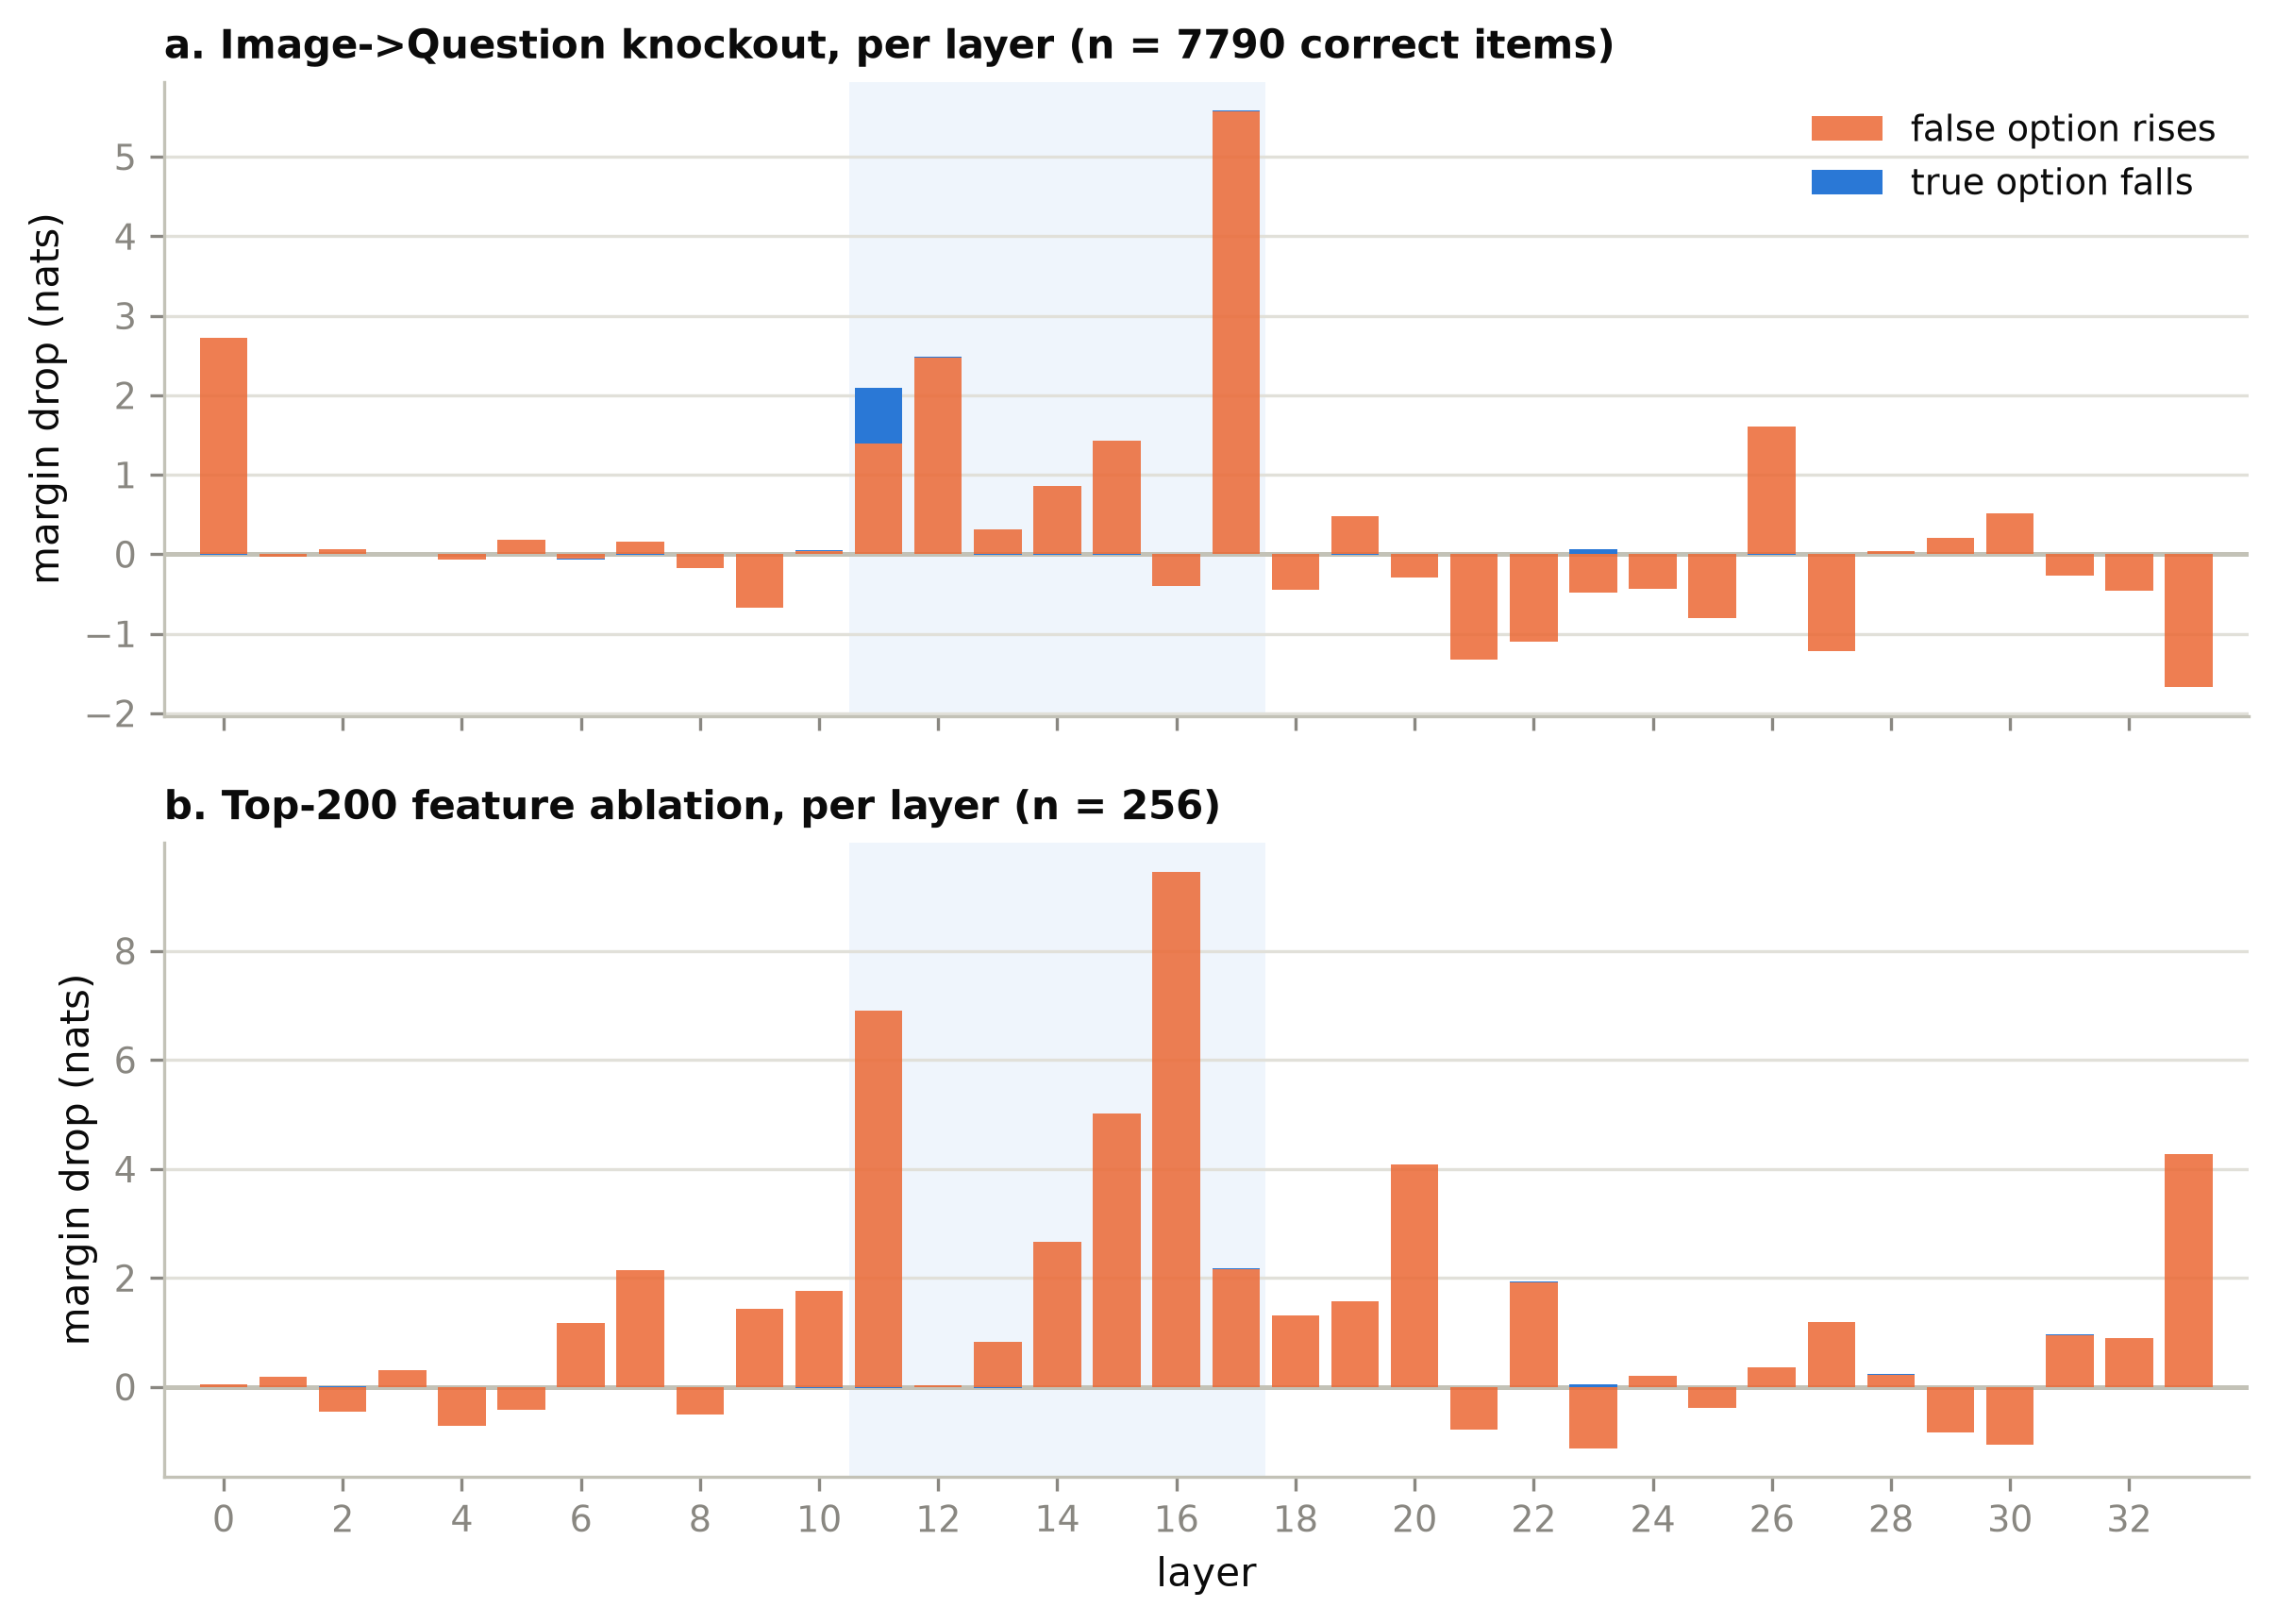
\includegraphics[width=\textwidth]{gemma3_4b_fig_decomposition}
  \caption{\textbf{What the margin drop is made of.} Per-layer margin drop
  split into the true option's loss (blue) and the false option's rise
  (orange), for Image$\rightarrow$Question knockout (a; $n = 7,790$)
  and top-200 feature ablation (b; $n = 256$). Apart from the knockout at
  layer 11, no single-layer intervention of either kind moves the true
  option.}
  \label{fig:gemma-decomp}
\end{figure}

\paragraph{The joint ablation removes more than the pathway.} Ablating 200
features at each of layers 11--17 drops the margin by 28.6 against 23.5 for the
seven-layer knockout, $R = 1.22$ (95\% CI $[1.18, 1.26]$); across the nested
spans $R$ runs from 0.40 to 2.28 and rises with span size (slope $+0.044$ per
layer, 95\% CI $[+0.031, +0.056]$), the signature the LLaVA analysis treated as
evidence of compensation. Here it means something else. The joint ablation
takes the true option from $-0.05$ to $-10.1$ nats and generation accuracy
from 0.996 to 0.000: the model stops answering the question, emitting
\texttt{okay} on 174 of 256 items and \texttt{based}, \texttt{this} or
\texttt{the} on most of the rest. The seven-layer knockout, which removes
strictly all image information those layers could carry, leaves the model
answering in the task's vocabulary with the true option at $-1.0$. An
intervention that exceeds the ceiling at the same locus is not recovering the
pathway; it is removing computation the pathway's ceiling never contained. The
features the margin gradient selects at the attention output are, on the
evidence of what the model then produces, the ones that hold the answer
format and the task, not the ones that carry the image, and the isolation
condition in Appendix~\ref{app:gemma} --- ablation with
Image$\rightarrow$Question severed at every layer --- tests that directly.

\paragraph{The budget results reverse.} The concentrated curve at layer 17 is
not flat: from $k = 40$ to 800 the drop rises from 0.68 to 6.19, close to
linearly in $k$, with the true option unmoved throughout
(Figure~\ref{fig:gemma-budget}). The spread allocation ($40 \times 7 = 280$
features) drops the margin by 23.8 against 2.99 for $k = 280$ concentrated,
$7.97\times$ --- but it does so by destroying the answer (accuracy 0.008),
which no concentrated budget does. The equal-budget contrast that on LLaVA
separated allocation from size here separates ``many features at one site,
harmless'' from ``few features at many sites, catastrophic'', and the matched
random spread control (0.69) shows the catastrophe is feature-specific. The
downstream test also reverses: with Image$\rightarrow$Question blocked at
layers 18--33 the layer-17 ablation adds nothing to the knockout (combined
14.92 against 14.94 alone, and 2.17 for the ablation by itself), where on
LLaVA the two were additive to 0.4\%. Leave-one-out marginal contributions
are 0.01--0.57 of the standalone effects, the redundancy signature, but at a
floor: the joint condition has already removed the answer, and no single
layer's return changes that.

\begin{figure}[t]
  \centering
  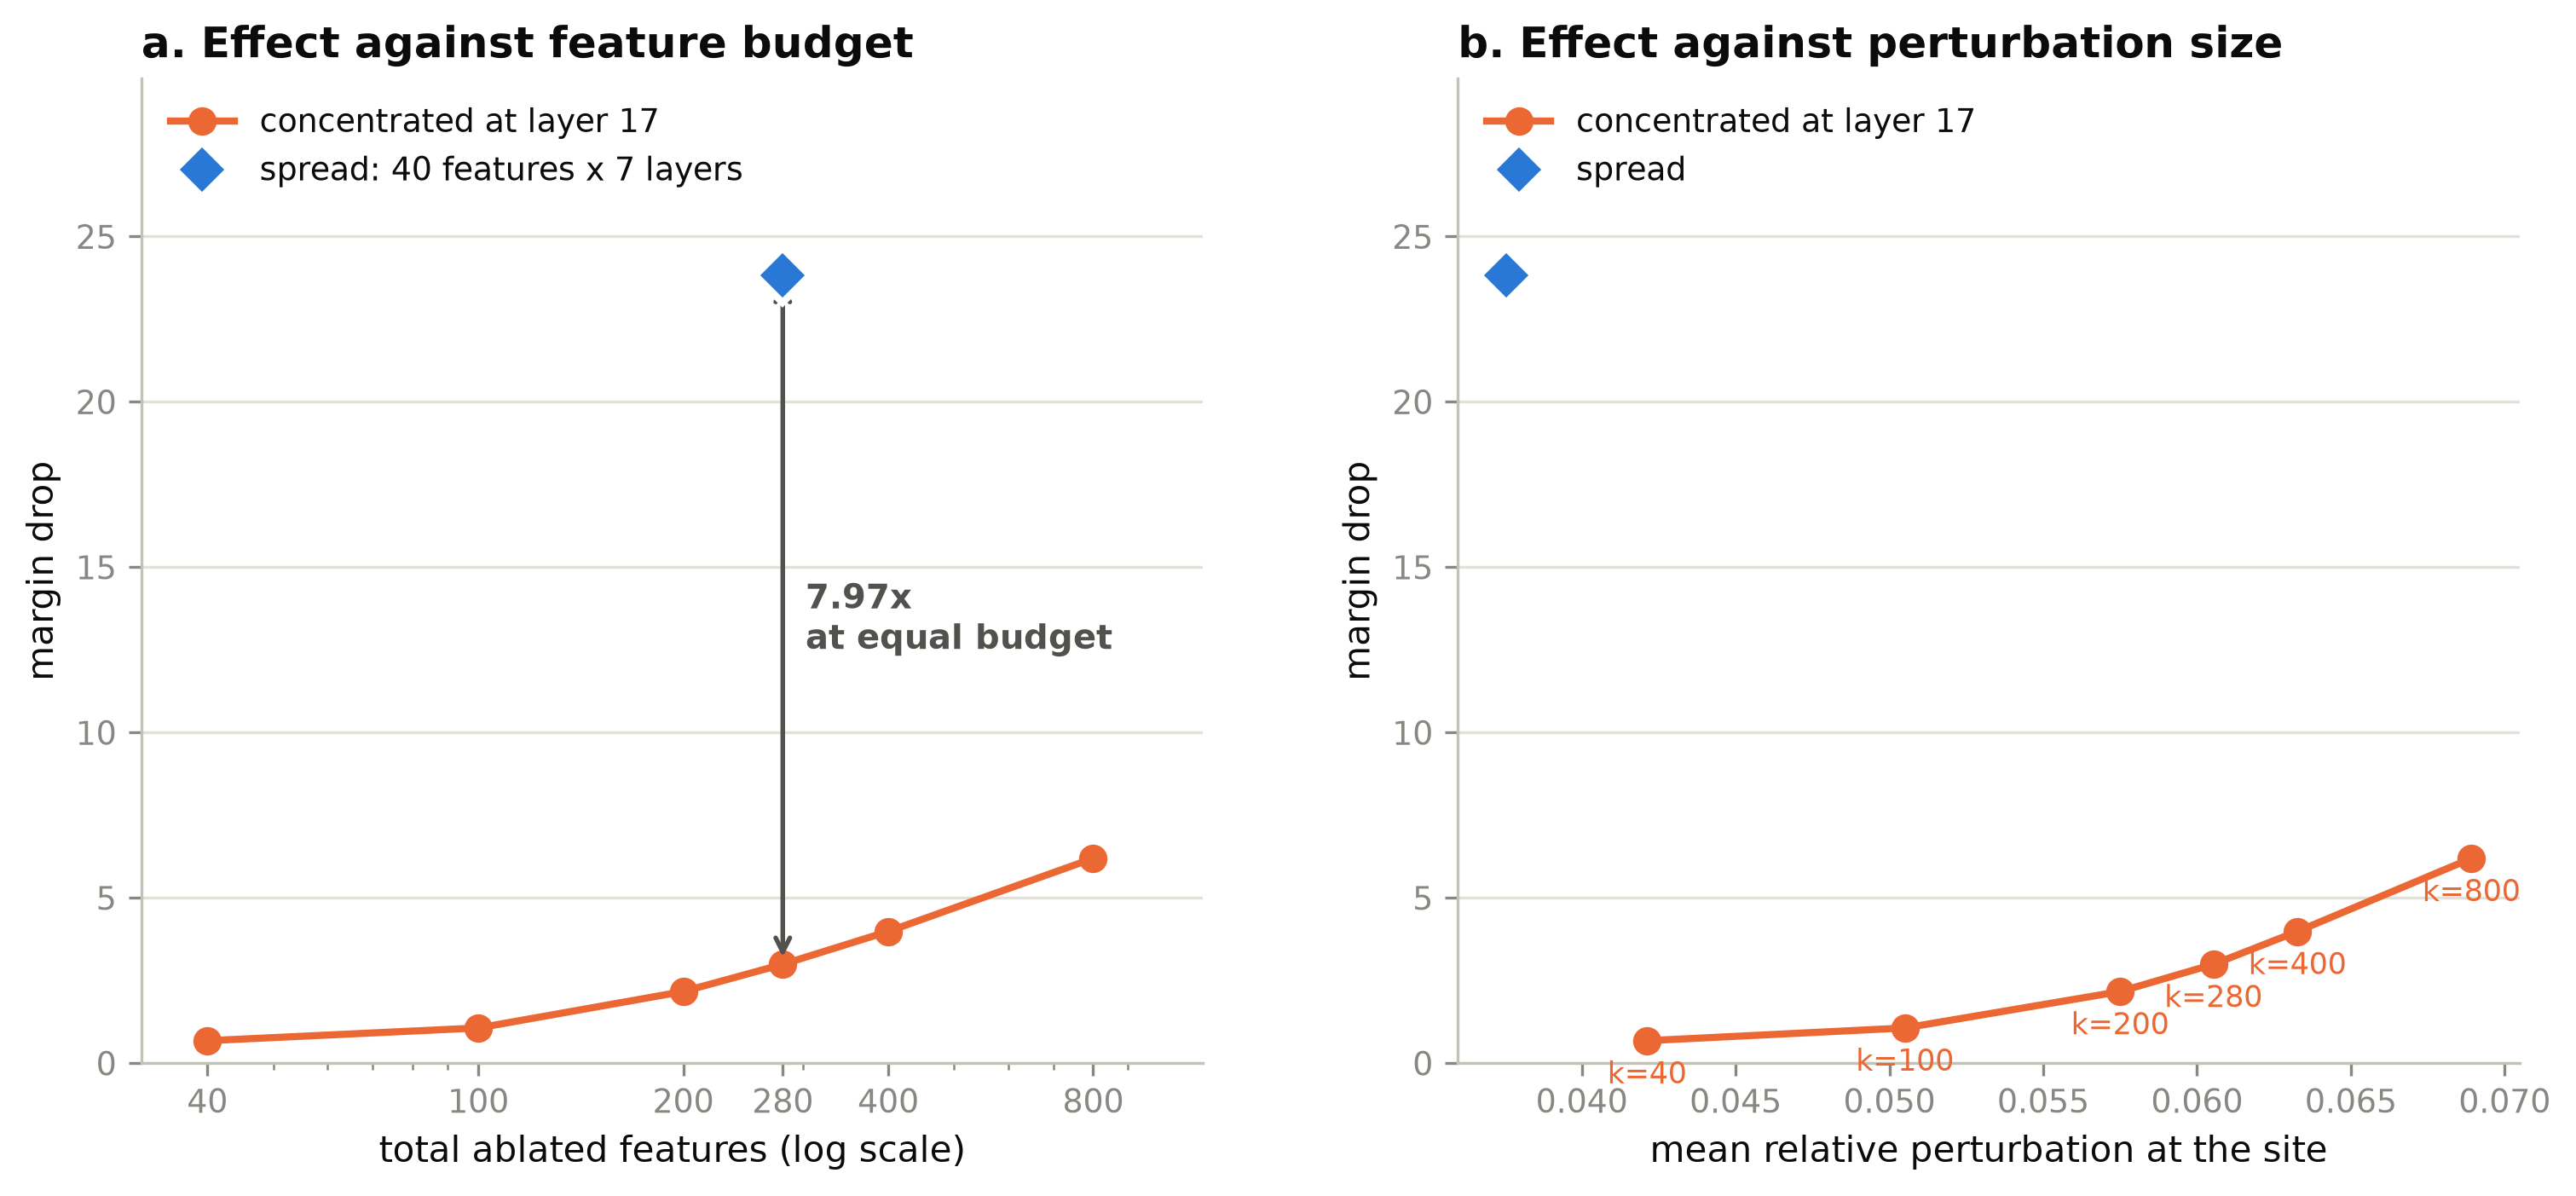
\includegraphics[width=\textwidth]{gemma3_4b_fig6_budget_distribution}
  \caption{\textbf{Budget and allocation on Gemma~3.} (a) Margin drop against
  total ablated features for a budget concentrated at layer 17
  ($k = 40$--$800$) and spread across layers 11--17 (40 per layer). (b) The
  same against the mean relative perturbation of the site. The concentrated
  curve grows with $k$ and never reaches the answer; the spread point reaches
  it by ending the model's participation in the task.}
  \label{fig:gemma-budget}
\end{figure}

\paragraph{What transfers.} The instrument transfers: the adapter passed the
same contract checks, the knockout reached both the sliding-window and the
global layers, the null interventions returned exactly zero, and the matrix
ran unchanged. The calibration does not, and the reasons are diagnosable from
the numbers the design already produces. A pass-through drop of the size of an
effect says the dictionary is not the model's basis at that site. An ablation
above the knockout ceiling says the features act off the pathway. A margin
drop with no true-option loss says the metric is measuring the tail. Each is a
precondition the LLaVA study met silently, and the recommendation this adds to
the paper's is that they be checked and reported: the pass-through in
\texttt{replace} mode, $A/K$ per single layer, and the true-option component
of every effect. On the dictionaries themselves: a text-trained SAE applied to
a vision-language model's attention output is a different instrument from one
trained on the multimodal activations, whatever its width, and the $L_0$ it
reaches on the task (75--169 here, against a nominal 60--120) is the first
sign.

% ============================================================
% Standalone only: inside main_final.tex, \appendix has already been issued
% after Appendix D and a second call would restart the lettering at A.
\ifdefined\gemmastandalone\appendix\fi
% (append after Appendix D)
\section{Gemma 3: configuration and per-layer results}
\label{app:gemma}

\paragraph{Conventions.} Prompts use the model's chat template with the same
question and single-word-answer suffix; the processor materialises
\texttt{\textbackslash n\textbackslash n<start\_of\_image>}, 256 image tokens
and \texttt{<end\_of\_image>\textbackslash n\textbackslash n} in the sequence
(286 tokens), and \texttt{token\_type\_ids} are passed so the image block keeps
its bidirectional attention. The image is encoded once per question and its
features are scattered into the token embeddings for every subsequent pass,
the model's own path, verified to reproduce the pixel path. The model runs in
bfloat16 with an untied float32 copy of the language-model head. On the first
32 validation items the model generated \texttt{Blue}, \texttt{Square},
\texttt{Yellow} without exception; \texttt{Blue} scores $0.00$ nats,
\texttt{blue} $-16.5$, and \texttt{" blue"} $-19.9$, so both options of every
pair are capitalised before scoring. The knockout edits the materialised 4D
attention mask as before; transformers~4.57 hands both the sliding-window
and the global layers such a mask under eager attention, and the edit was
verified to move the margin at layer 0 (sliding) and layer 5 (global). One
A100-40GB per job: 0.10\,s per language-model forward, 17\,h per flow for the
sweep, 2\,h\,39\,m for the 57-condition matrix.

\begin{table}[h]
  \centering
  \caption{Gemma~Scope~2 attention dictionaries on the task's activations
  (validation split, question positions, 203{,}245 rows per layer). Nominal
  $L_0$ is the release's target; the rest is measured here. Explained variance
  for the LLaVA dictionaries in Table~\ref{tab:sae} was 0.9985--0.9998.}
  \label{tab:gemma-sae}
  \small
  \begin{tabular}{rrrrr@{\hskip 1.5em}rrrrr}
    \toprule
    Layer & Nom.\ $L_0$ & Expl.\ var. & $L_0$ & Dead & Layer & Nom.\ $L_0$ & Expl.\ var. & $L_0$ & Dead \\
    \midrule
     0 &  60 & 0.788 & 160.4 & 0.70 & 17 & 120 & 0.813 & 140.8 & 0.61 \\
     1 &  65 & 0.821 &  78.9 & 0.79 & 18 & 120 & 0.826 & 128.9 & 0.68 \\
     2 &  70 & 0.857 &  81.0 & 0.82 & 19 & 120 & 0.805 & 116.7 & 0.66 \\
     3 &  75 & 0.831 &  74.9 & 0.85 & 20 & 120 & 0.784 & 112.3 & 0.74 \\
     4 &  81 & 0.822 &  82.4 & 0.86 & 21 & 120 & 0.771 & 105.6 & 0.65 \\
     5 &  86 & 0.847 & 114.6 & 0.80 & 22 & 120 & 0.788 & 121.7 & 0.65 \\
     6 &  91 & 0.761 &  96.9 & 0.79 & 23 & 120 & 0.787 & 166.4 & 0.46 \\
     7 &  97 & 0.790 & 108.8 & 0.84 & 24 & 120 & 0.829 & 112.7 & 0.58 \\
     8 & 102 & 0.780 & 110.9 & 0.79 & 25 & 120 & 0.751 & 133.8 & 0.65 \\
     9 & 107 & 0.823 & 121.6 & 0.79 & 26 & 120 & 0.740 & 169.4 & 0.48 \\
    10 & 112 & 0.740 & 128.1 & 0.76 & 27 & 120 & 0.950 & 106.1 & 0.64 \\
    11 & 118 & 0.786 & 107.8 & 0.69 & 28 & 120 & 0.815 & 134.2 & 0.70 \\
    12 & 120 & 0.828 & 130.2 & 0.71 & 29 & 120 & 0.869 & 113.7 & 0.59 \\
    13 & 120 & 0.763 & 124.5 & 0.65 & 30 & 120 & 0.807 & 123.1 & 0.66 \\
    14 & 120 & 0.777 & 149.5 & 0.60 & 31 & 120 & 0.668 & 113.0 & 0.68 \\
    15 & 120 & 0.768 & 135.3 & 0.53 & 32 & 120 & 0.794 & 156.6 & 0.69 \\
    16 & 120 & 0.805 & 151.6 & 0.68 & 33 & 120 & 0.688 & 135.5 & 0.62 \\
    \bottomrule
  \end{tabular}
\end{table}

\paragraph{Pass-through in \texttt{replace} mode.} With no features ablated,
substituting the reconstruction for the activation at every question position
moves the margin by $+1.56$ (layers 11--17), $+1.52$ (12--17), $+1.39$
(13--17), $+0.61$ (14--17), $+0.50$ (15--17), $-1.58$ (16--17) and $-0.90$
(layer 17 alone), at a relative perturbation of the site of 0.037--0.042. In
delta mode the same conditions give $0.0000$, and the no-hook condition gives
$0.0$.

\begin{table}[h]
  \centering
  \caption{Ablation $A$ and knockout $K$ on the same 256 questions, per span
  layer and per span, with paired bootstrap intervals on $R = A/K$ (10{,}000
  resamples). Single-layer $A$ is the top-200 delta-mode ablation; ``ctl'' is
  the mean of 15 activation-matched random sets. $R$ is undefined at layer 16,
  whose knockout is inhibitory. True-option loss is the part of the drop due
  to the true option's log-probability falling.}
  \label{tab:gemma-spans}
  \small
  \begin{tabular}{llrrrrrl}
    \toprule
    & Layer / span & $A$ & ctl & $K$ & $R$ & true loss $A$ / $K$ & 95\% CI on $R$ \\
    \midrule
    \multirow{7}{*}{Single}
      & 11 & 6.883 & 0.28 &  2.458 & 2.80 & $-0.01$ / 0.97 & --- \\
      & 12 & 0.037 & 0.07 &  2.552 & 0.01 & $-0.00$ / $-0.00$ & --- \\
      & 13 & 0.819 & $-0.02$ & 0.291 & 2.82 & $-0.01$ / $-0.00$ & --- \\
      & 14 & 2.662 & $-0.06$ & 0.891 & 2.99 & $-0.00$ / $-0.00$ & --- \\
      & 15 & 5.020 & 0.19 &  1.364 & 3.68 & $+0.01$ / $-0.00$ & --- \\
      & 16 & 9.454 & 0.25 & $-0.397$ & --- & $-0.00$ / $+0.00$ & --- \\
      & 17 & 2.166 & 0.29 &  5.427 & 0.40 & $+0.01$ / $-0.01$ & [0.343, 0.456] \\
    \midrule
    \multirow{6}{*}{Nested}
      & \{16,17\}  & 10.866 & 0.53 &  5.101 & 2.13 & 0.01 / 0.00 & [1.990, 2.287] \\
      & \{15--17\} & 14.168 & 0.76 &  6.227 & 2.28 & 0.40 / $-0.00$ & [2.129, 2.437] \\
      & \{14--17\} & 14.631 & 0.66 &  8.962 & 1.63 & 0.41 / $-0.01$ & [1.556, 1.715] \\
      & \{13--17\} & 16.013 & 0.82 &  9.269 & 1.73 & 1.04 / $-0.02$ & [1.642, 1.819] \\
      & \{12--17\} & 24.678 & 0.93 & 13.716 & 1.80 & 12.79 / 0.02 & [1.730, 1.872] \\
      & \{11--17\} & 28.609 & 1.14 & 23.548 & 1.22 & 10.02 / 0.95 & [1.176, 1.256] \\
    \midrule
    \multirow{2}{*}{Size 3}
      & \{11,12,13\} & 11.920 & 0.26 &  9.259 & 1.29 & 1.19 / 1.09 & [1.128, 1.481] \\
      & \{11,13,15\} & 14.369 & 0.42 &  4.121 & 3.49 & 1.64 / 0.98 & [2.686, 4.678] \\
    \midrule
    Sensitivity & \{11--15,17\} & 27.170 & --- & 23.024 & 1.18 & 9.72 / 1.16 & [1.139, 1.224] \\
    \bottomrule
  \end{tabular}
\end{table}

\paragraph{Downstream and leave-one-out.} Anchor 17: ablation 2.166,
Image$\rightarrow$Question knockout at layers 18--33 alone 14.944, combined
14.924 (additive prediction 17.110; excess $-2.19$). Anchor 12: 0.054, 28.893,
28.804 (prediction 28.947). Leave-one-out marginal contributions to the joint
28.609, against standalone effects: layer 11, $+3.93$ vs 6.88; 12, $+3.45$ vs
0.04; 13, $-0.04$ vs 0.82; 14, $+0.95$ vs 2.66; 15, $+0.04$ vs 5.02; 16,
$+1.44$ vs 9.45; 17, $+0.64$ vs 2.17. Every leave-one-out condition leaves
generation accuracy at or below 0.004.

\paragraph{Isolation.} With Image$\rightarrow$Question blocked at all 34 layers
the model is at chance on the forced choice (margin $-0.20$, accuracy 0.473;
true option $-6.09$, false $-5.89$) and still answers in the task's
vocabulary (\texttt{circle}, \texttt{red}, \texttt{blue}). Ablating the top-200
features of one span layer on top of that changes the margin by at most 0.32
--- there is no image information left to remove --- but still moves the
true option: by $-1.30$ nats at layer 16, whose ablation also turns 113 of the
256 generations into \texttt{it}, and by $+0.76$, $-0.32$, $-0.71$, $+0.68$,
$+0.16$ and $+0.13$ at layers 11 through 15 and 17. The joint ablation with no
image reachable takes the true option from $-6.09$ to $-9.52$ and every one of
the 256 generations to \texttt{this}. A third of the true-option loss the joint
ablation inflicts with the image present (10.0 nats) is therefore inflicted
with the image absent, and the collapse of the output format is complete in
both cases: the selected features are, to that extent, not on the pathway the
knockout measures.

\paragraph{Per-layer ablation outside the span.} Figure~\ref{fig:gemma-single}
gives the top-200 delta-mode ablation at every layer with its matched
controls. Outside the span the largest effects are at layers 20 (4.08), 33
(4.26), 7 (2.13) and 22 (1.93); negative effects (ablation raises the margin)
occur at layers 2, 4, 5, 8, 21, 23, 25, 29 and 30. None moves the true option
by more than 0.05 nats.

\begin{figure}[h]
  \centering
  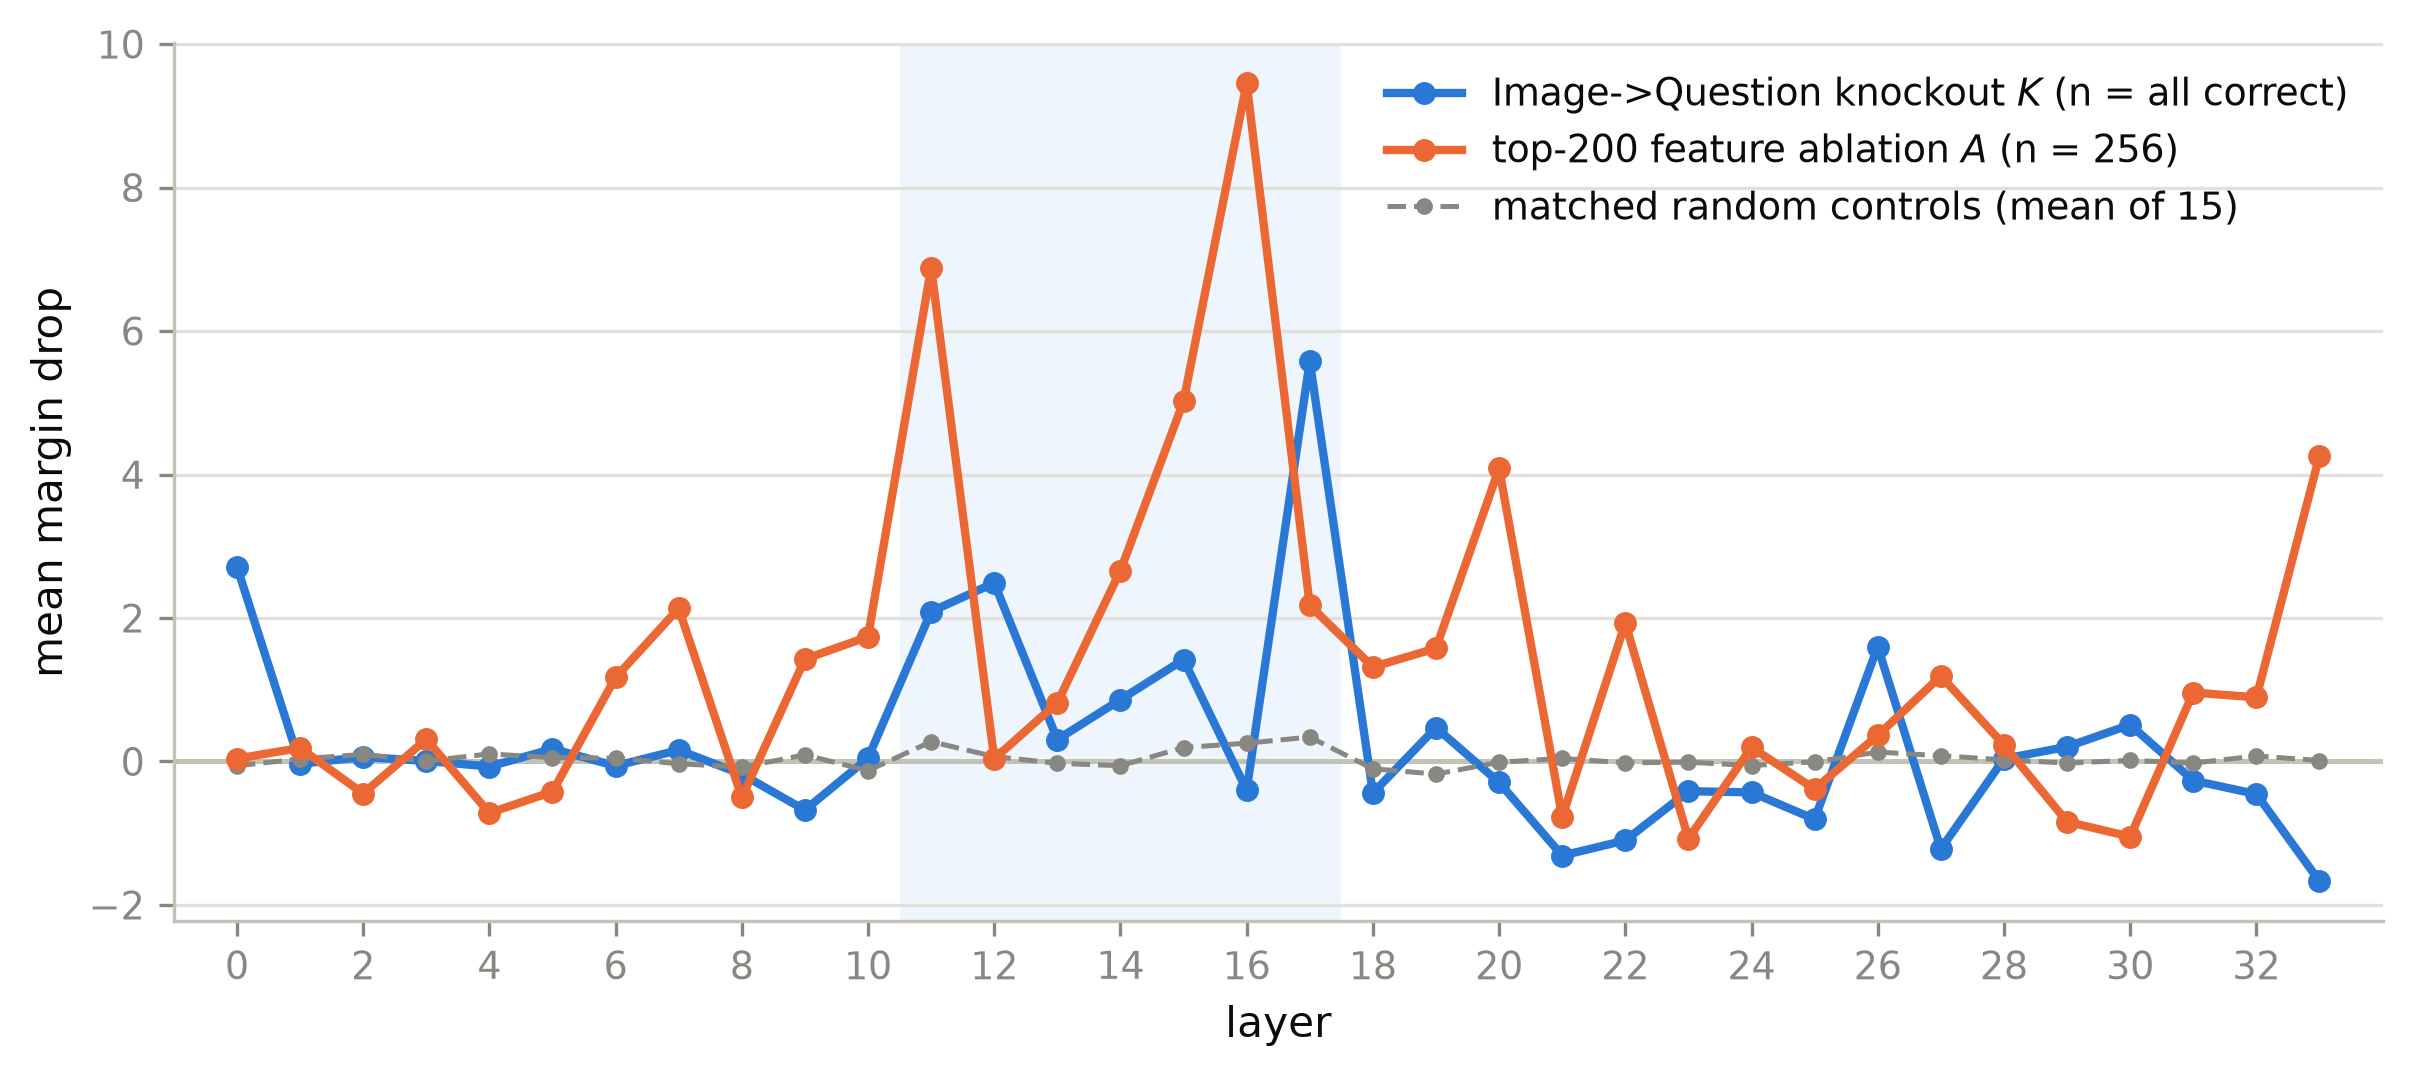
\includegraphics[width=\textwidth]{gemma3_4b_fig_single_layer}
  \caption{Top-200 delta-mode feature ablation at each of the 34 layers
  ($n = 256$) with the mean of 15 activation-matched random controls, and the
  Image$\rightarrow$Question knockout on the correctly answered validation set
  for comparison.}
  \label{fig:gemma-single}
\end{figure}

\begin{figure}[h]
  \centering
  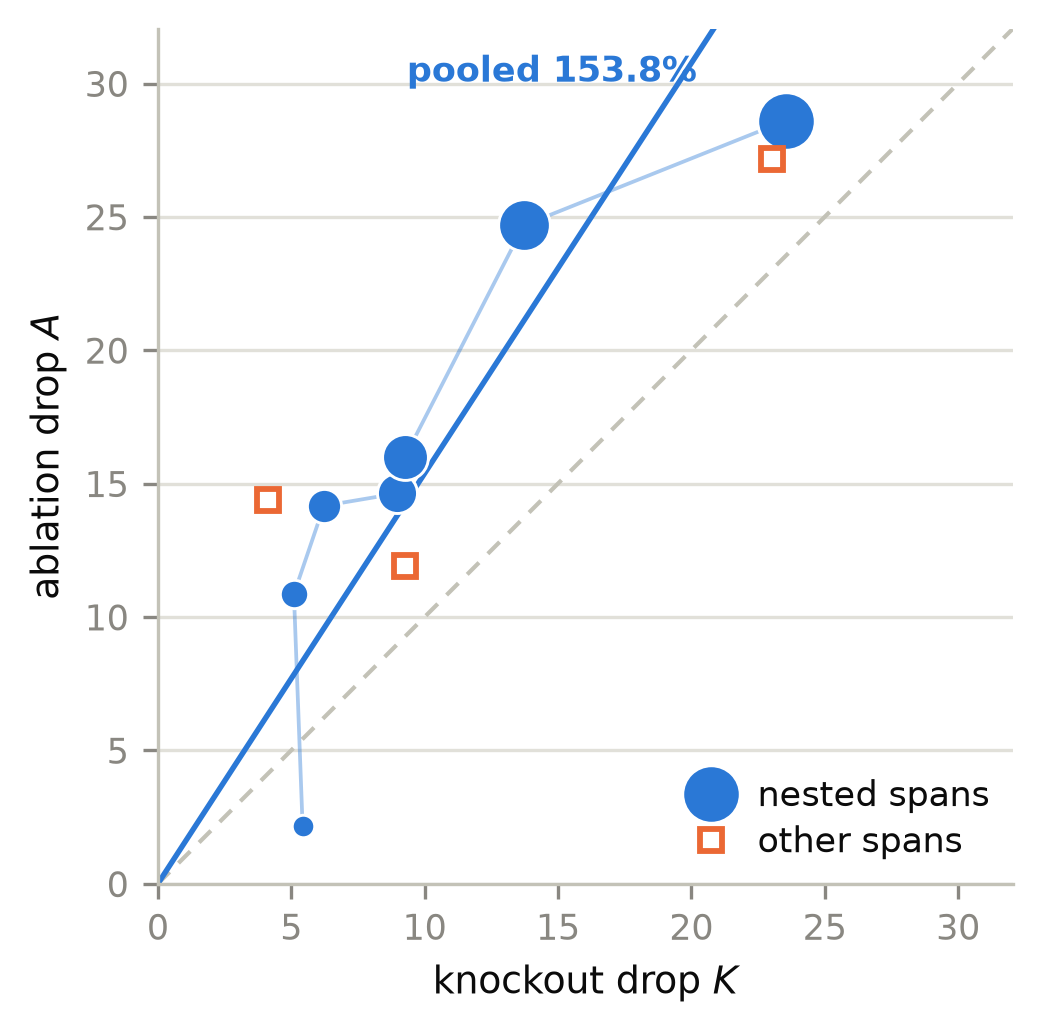
\includegraphics[width=0.58\textwidth]{gemma3_4b_fig8a_ablation_vs_knockout}
  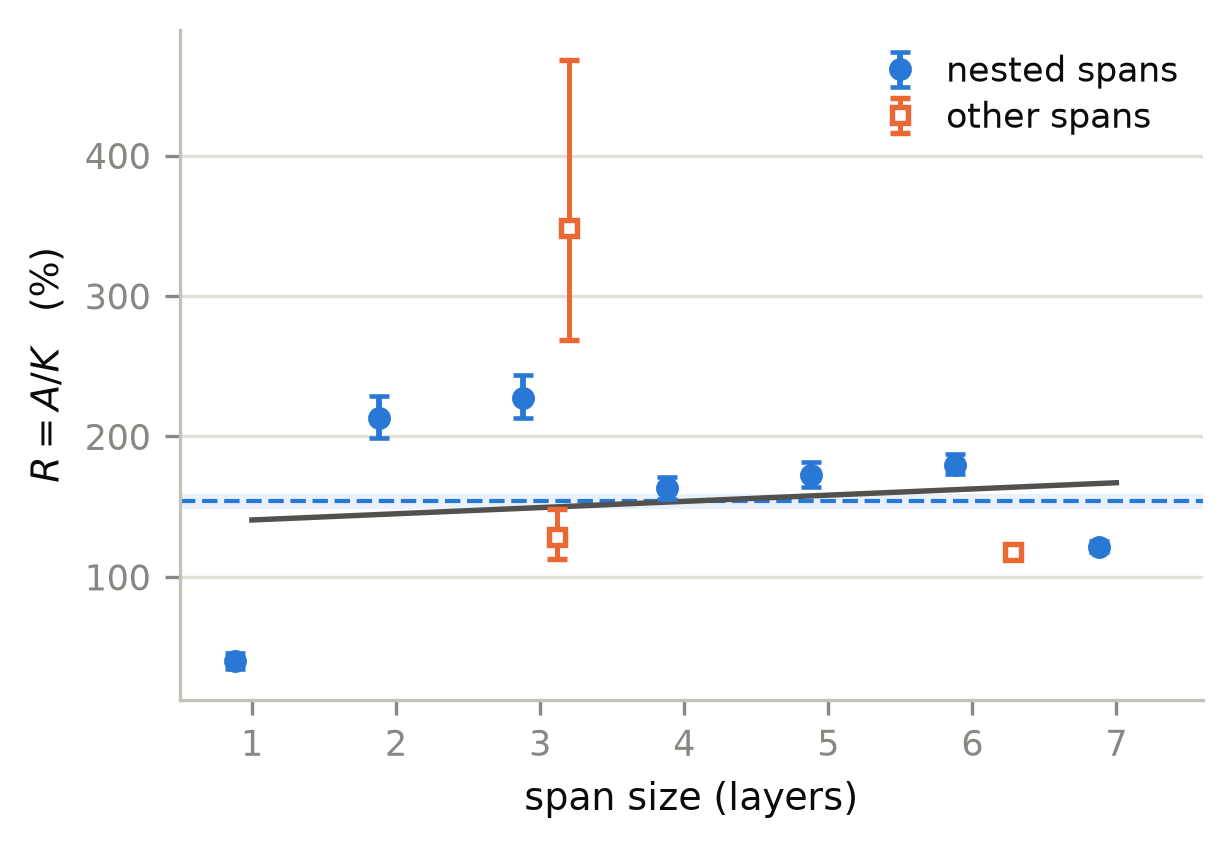
\includegraphics[width=0.66\textwidth]{gemma3_4b_fig8b_recovered_share}
  \caption{The LLaVA span figures (Figures~\ref{fig:scaling}
  and~\ref{fig:rshare}) redrawn for Gemma~3. Every multi-layer span lies above
  parity, and $R$ rises with span size; read with
  Figure~\ref{fig:gemma-decomp} and the generation accuracies in the text,
  this is the joint ablation removing the model's participation in the task
  rather than recovering more of the pathway.}
  \label{fig:gemma-spans}
\end{figure}

\ifdefined\gemmastandalone
  \bibliographystyle{plainnat}
  \bibliography{refs}
  \expandafter\enddocument
\fi

% ============================================================
% refs.bib additions -- ALREADY APPENDED to refs.bib; kept here for the record
% ============================================================
% @article{gemma3,
%   title   = {Gemma 3 Technical Report},
%   author  = {{Gemma Team} and Kamath, Aishwarya and Ferret, Johan and Pathak, Shreya and others},
%   journal = {arXiv preprint arXiv:2503.19786},
%   year    = {2025}
% }
% @techreport{gemmascope2,
%   title       = {Gemma Scope 2 --- Technical Paper},
%   author      = {McDougall, Callum and Conmy, Arthur and Kram{\'a}r, J{\'a}nos and Lieberum, Tom and Rajamanoharan, Senthooran and Nanda, Neel},
%   institution = {Google DeepMind},
%   year        = {2025},
%   note        = {Weights at \url{https://huggingface.co/google/gemma-scope-2-4b-it}}
% }
% @article{rajamanoharan2024jumprelu,
%   title   = {Jumping Ahead: Improving Reconstruction Fidelity with {JumpReLU} Sparse Autoencoders},
%   author  = {Rajamanoharan, Senthooran and Lieberum, Tom and Sonnerat, Nicolas and Conmy, Arthur and Varma, Vikrant and Kram{\'a}r, J{\'a}nos and Nanda, Neel},
%   journal = {arXiv preprint arXiv:2407.14435},
%   year    = {2024}
% }
%
% ============================================================
% Suggested edits elsewhere in main_final.tex (for the author to apply)
% ============================================================
% Abstract, after "...is not evidence that the selected features account for
% the mechanism.": "A replication on Gemma 3 4B with Gemma Scope 2's
% pre-trained attention dictionaries finds the calibration's three
% preconditions -- a dictionary that fits the site, features that act on the
% pathway, and a margin far from saturation -- all violated, and shows the
% numbers by which each violation is detected."
%
% Limitations paragraph: replace "Results come from one model, one synthetic
% task, one dictionary placement and one seed per layer" with "The positive
% results come from one model, one synthetic task, one dictionary placement
% and one seed per layer; the Gemma 3 replication (Section~\ref{sec:gemma})
% shows what the same design returns when its preconditions fail, and does
% not establish that they can be met with pre-trained dictionaries."
%
% Availability: add "and the Gemma 3 runs, adapter and configurations at
% https://github.com/KremerML/vlm-flow-probe".
